{\chapter{Background}
\label{chap:Background}

In this chapter, we are presenting the necessary background knowledge concerning topics covered in this thesis. In (\ref{sec:Graphs}), we define what is a graph according to the graph theory and discuss the different graph types. In (\ref{sec:GraphModels}), we discuss the property graph model (PGM) and the resource description framework model (RDF), as two types of logical graph data models that are mostly used by state of the art graph databases. We present the storage structures used by graph databases to store graph data in (\ref{sec:StorageStructures}). We end the chapter with a summary of what have been discussed in the chapter (\ref{sec:BackgroundSummary}).

\section{Graphs}
\label{sec:Graphs}
In this section, we discuss graphs and graph  types. In (\ref{subsec:Graph?}), we adopt a clear definition for graphs. A definition that is based on the graph theory. In (\ref{subsec:GraphTypes}), we state the different types of graphs. A graph type is a factor that must be taken into consideration in the storage and retrieval methods of the graph.

\subsection{What is a Graph?}
\label{subsec:Graph?}
Graph theory is a mathematical topic that is focused on the study of graphs. A graph \textit{G} is defined as a finite nonempty set \textit{V} of vertices along with the set \textit{E} of edges. The set \textit{E} consists of unordered pairs of vertices in \textit{V}, where an edge \textit{x \(\in\) E} is defined as a pair of vertices \(\textit{x=\{u,v\}}\) \cite{harary6graph}.

We define any two vertices \textit{u \(\in\) V} and \textit{v \(\in\) V} that forms any of the edges in \textit{E} as adjacent vertices. Similarly, two edges \textit{x \(\in\) E} and \textit{y \(\in\) E} are adjacent if they are formed of two pair of vertices where the two pair are sharing one common vertex. The adjacencies of a vertex \textit{u}, is the set \textit{K \(\in\) V} of vertices, where for each vertex \textit{a \(\in\) K}, there is an edge \textit{s \(\in\) E} and \textit{s=\{u,a\}} \cite{harary6graph}.

\begin{figure}
\centering
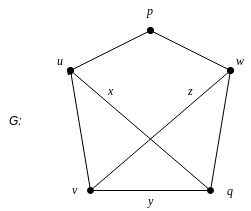
\includegraphics{pics/Graph.png}
\caption{An example of a graph \textit{G} \cite{harary6graph}}
\label{fig_graph}
\end{figure} 

In (\ref{fig_graph}), we are showing an example of a graph \textit{G}. In graph \textit{G}, vertices \textit{u} and \textit{v} are adjacent while vertices \textit{u} and \textit{w} are not. Similarly, edges \textit{x} and \textit{y} are adjacent while edges \textit{x} and \textit{z} are not. The adjacencies of vertex \textit{u} in the graph is the set of vertices \textit{\{p,v,q\}} \cite{harary6graph}.




\subsection{Graph Types}
\label{subsec:GraphTypes}

Graphs come in many types and shapes according to how rich they are with information. In (\ref{fig_graph-types}), we show an example of different graph types. A short explanation of each graph type is included in the below list. Some of the below mentioned graph types can be be used together to form one graph \cite{DBLP:journals/corr/abs-1006-2361}.


\begin{figure}
\centering
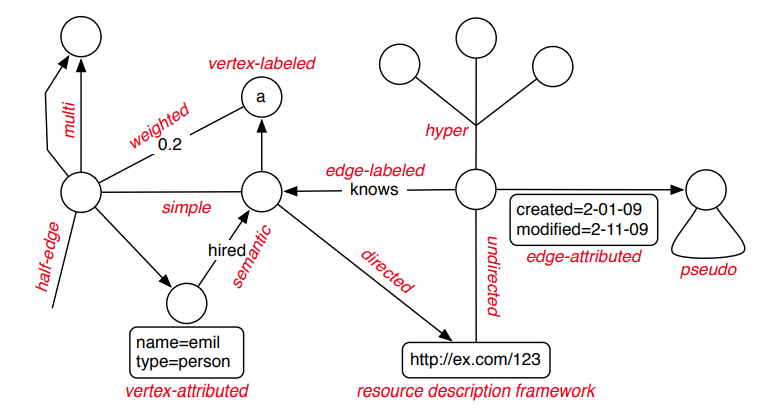
\includegraphics[width=16cm]{pics/graph-types.png}
\caption{An example of different graph types \cite{DBLP:journals/corr/abs-1006-2361}}
\label{fig_graph-types}
\end{figure} 

\begin{itemize}  
\item \textbf{Simple Graph:} a graph that permits no loops and only binary edges are allowed.

\item \textbf{Multi-graph:} a graph that allows the existence of more than one edge connecting the same two vertices.

\item \textbf{Pseudo Graph:} a graph with reflexive edges

\item \textbf{Weighted Graph:} a graph where a weight is assigned to edges to show the relationship strength.

\item \textbf{Semantic Graph:} used in semantic networks to model the relationships between concepts.

\item \textbf{Half-edge Graph:} an edge that is connected at one of its two ends to a vertex and on the other end connected to nothing.

\item \textbf{Hyper-graph:} a graph that permits an edge to connect more than one vertex.

\item \textbf{Directed Graph:} a graph where each edge is defined by an ordered pair of vertices (one of them is a source vertex and the other is a target vertex).

\item \textbf{Undirected Graph:} a graph where edges are denoting symmetric relationships between edges.

\item \textbf{Edge-labeled Graph:} used to specify the kind of relationship between vertices.

\item \textbf{Vertex-labeled Graph:} a graph where a label is assigned to a vertex to identify its type or identity.

\item \textbf{Edge-attributed Graph:} a graph where descriptive attributes are assigned to edges.

\item \textbf{Vertex-attributed Graph:} a graph where descriptive attributes are assigned to vertices.

\item \textbf{Resource Description Framework (RDF) Graph:} a graph where vertices and edges are identified by Uniform Resource Identifiers (URI). The RDF is a standard that was issued by the World Wide Web consortium.

\end{itemize}

\section{Graph Data Models}
\label{sec:GraphModels}

\subsection{Property Graph Model}
\label{subsec:PGM}
\subsection{Resource Description Framework (RDF) Model}
\label{subsec:RDF}


\section{Graph Storage Structures}
\label{sec:StorageStructures}

\subsection{Graph Topology}
\subsection{Graph Properties}


\section{Data Structures in C++}
\label{sec:DataStructuresInC++}

\subsection{Vector}
\subsection{Map}
\subsection{Unordered Map}

\section{Summary}
\label{sec:BackgroundSummary}

}